\documentclass[aspectratio=169]{beamer}
\usepackage{graphicx}
\usepackage[export]{adjustbox}

\title{Evolutionary Dynamics and Adaptation}
\subtitle{Genetic Impact of the Black Death\\
on Autoimmune Disorders}
\author{Krishna Vadali}
\date{August 2nd 2024}
\institute{Institute for Computing in Research}

\begin{document}

\frame{\titlepage}

\begin{frame}
  \frametitle{Contents}
  \begin{itemize}
      \item Introduction
      \item Choosing the gene
      \item Analyzing effectiveness and behavior
      \item Modern population 
      \item Future Work
  \end{itemize}
\end{frame}

\begin{frame}
  \frametitle{The Black Death}
  \centering
  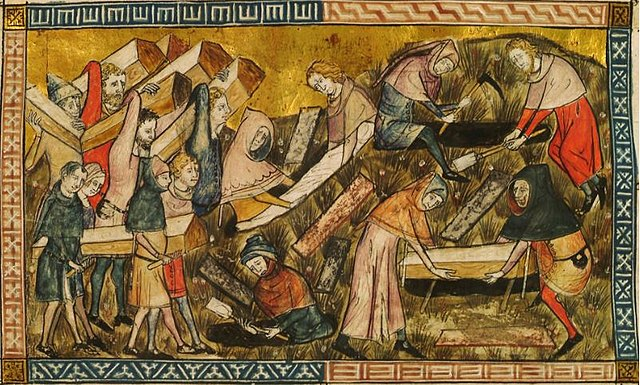
\includegraphics[width=0.8\textwidth]{images/black_death.jpg}
\end{frame}

\begin{frame}
\vspace{6mm}
  \frametitle{Pathogens and genes: Inter-Influence}
  \begin{figure}
      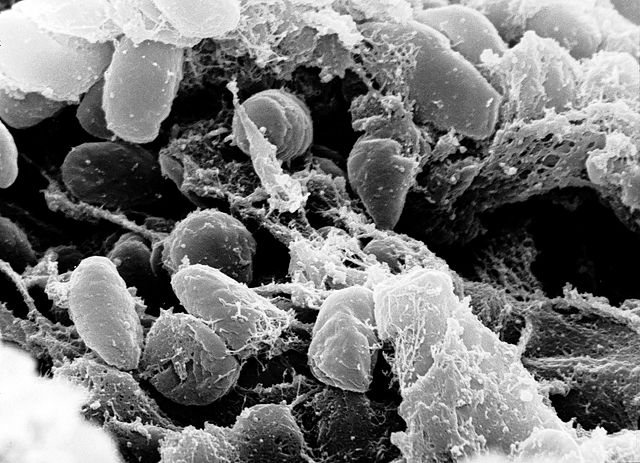
\includegraphics[width=0.30\textwidth]{images/pathogens.jpg}
      \caption{Y. Pestis}
  \end{figure}
  
  \begin{figure}
      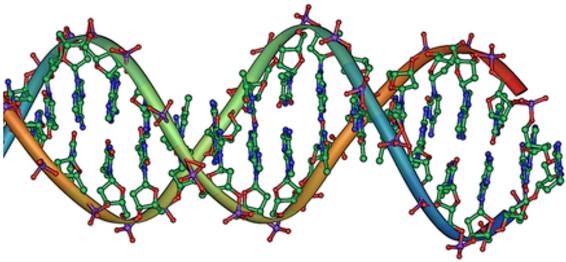
\includegraphics[width=0.30\textwidth]{images/dna.png}
      \caption{DNA}
  \end{figure}
\end{frame}

\begin{frame}
  \frametitle{SNPs}
  \centering
  \begin{figure}
    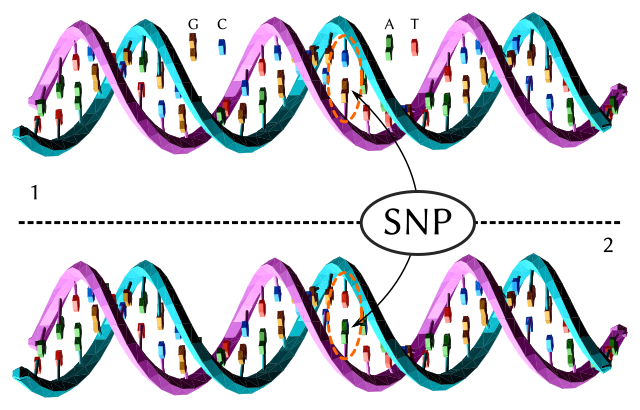
\includegraphics[width=0.7\textwidth]{images/snp.png}
    \caption{SNP}
  \end{figure}
\end{frame}

\begin{frame}
  \frametitle{Frequency of protection....}
  \centering
  \begin{figure}
    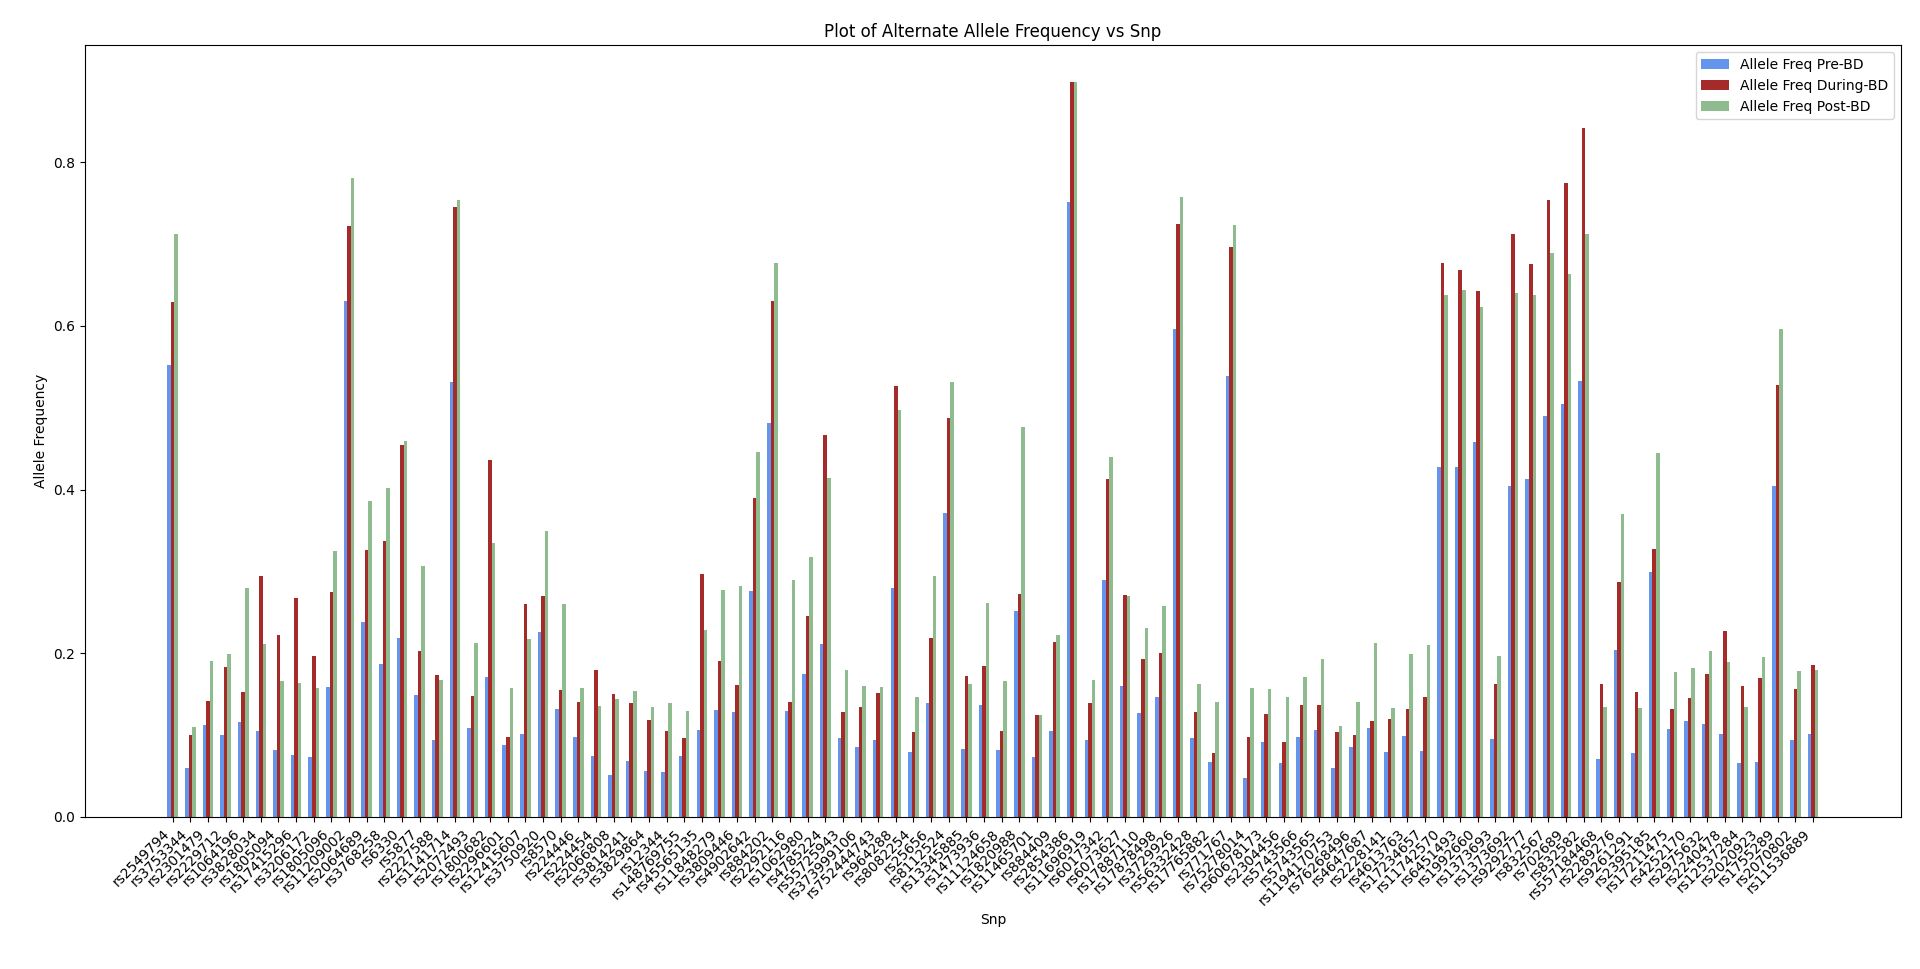
\includegraphics[width=1\textwidth]{images/snp-vs-allele-freq.png}
    \caption{Allele Frequency vs SNPs}
  \end{figure}
\end{frame}

\begin{frame}
  \frametitle{Genetic differentiation}
  \centering
  \begin{figure}
    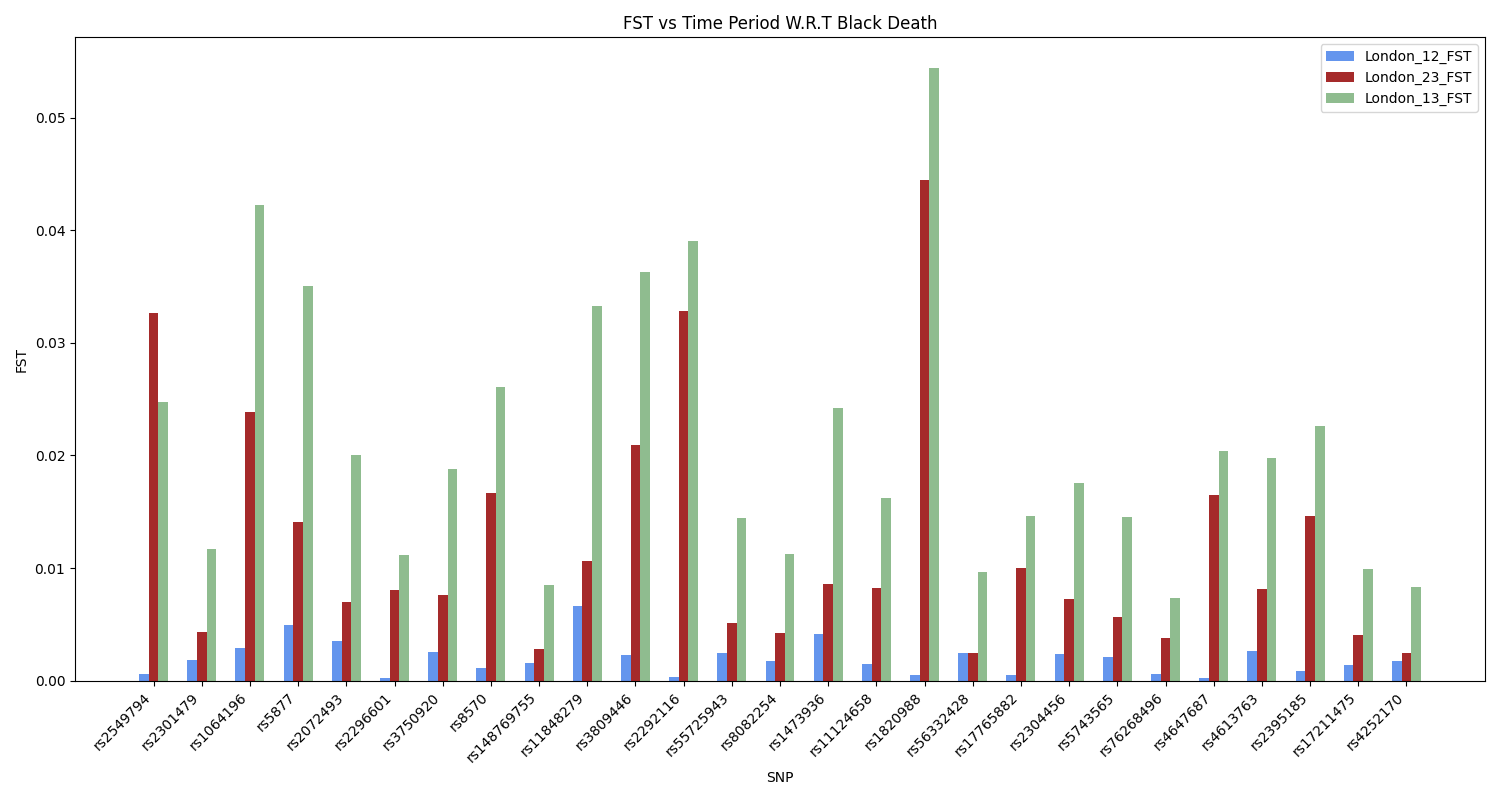
\includegraphics[width=0.8\textwidth]{images/snp-vs-fst.png}
    \caption{Fixation index vs SNP}
  \end{figure}
\end{frame}

\begin{frame}
  \frametitle{ERAP2 vs Cytokine Values under different Conditions}
  \centering
  \begin{figure}
    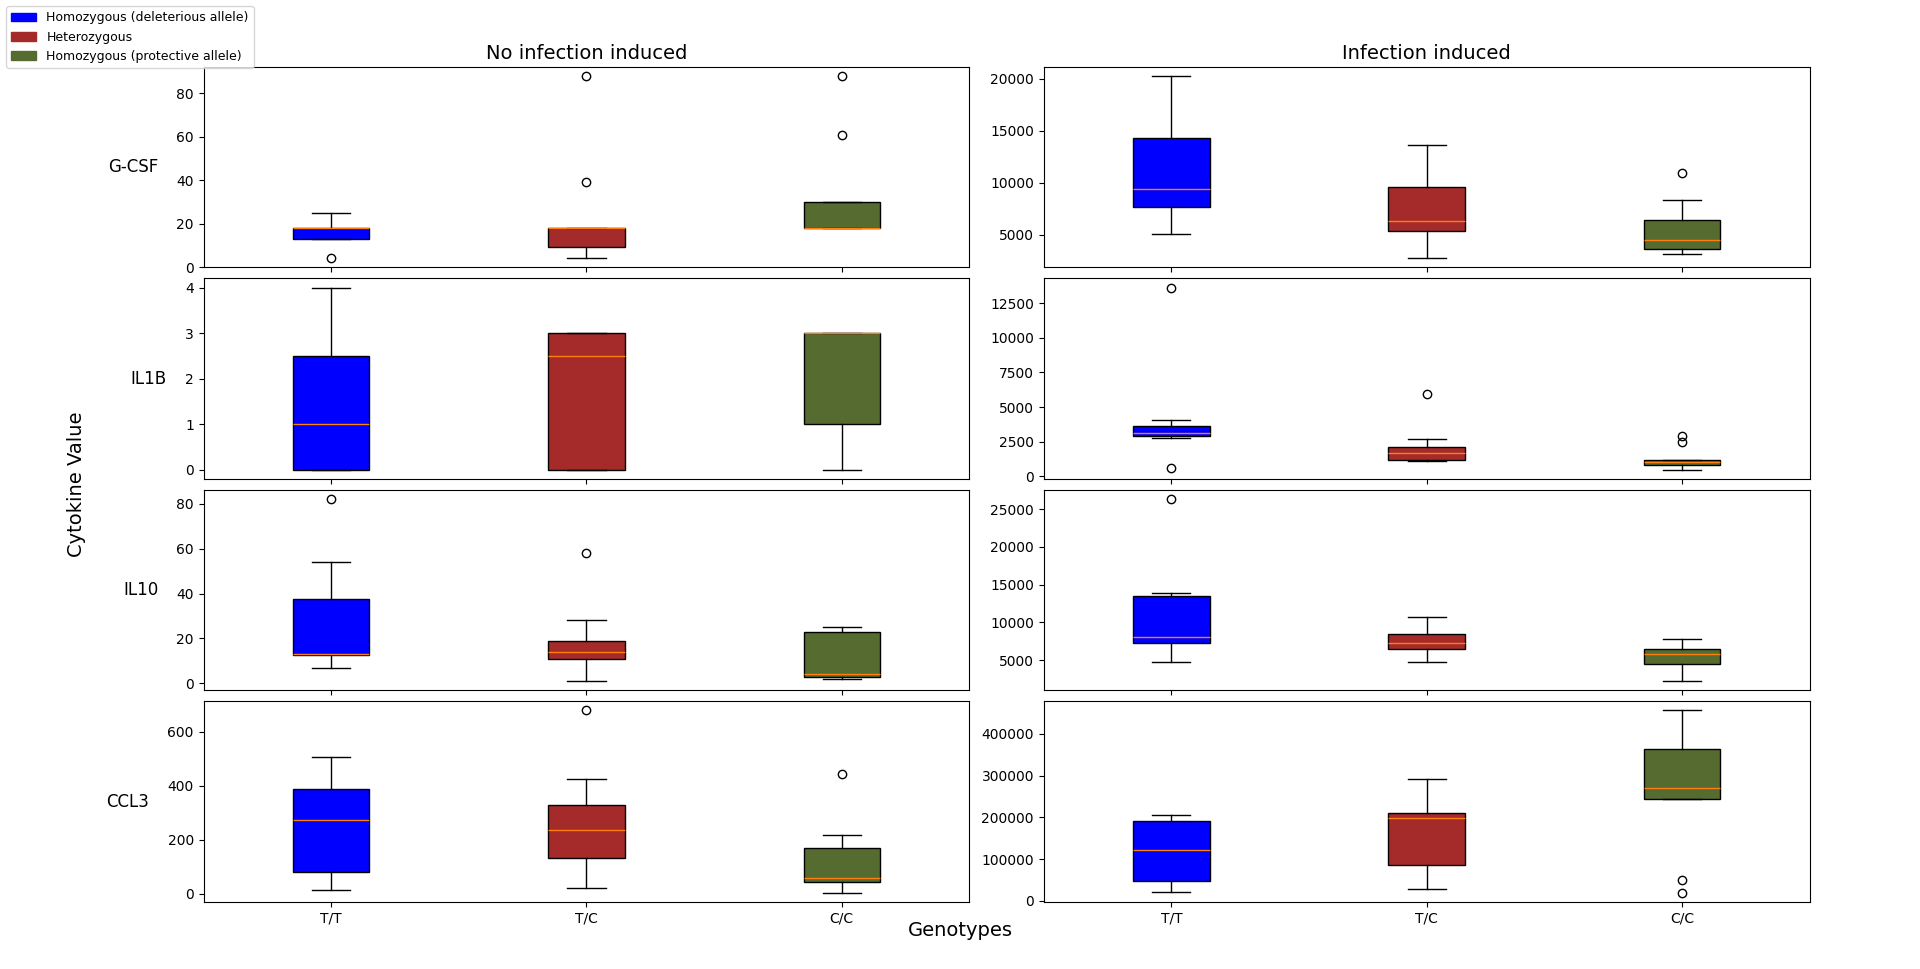
\includegraphics[width=1\textwidth]{images/boxplot.png}
    \caption{ERAP2 vs Cytokine Values}
  \end{figure}
\end{frame}

\begin{frame}
  \frametitle{Further look at infected data}
  \centering
  \begin{figure}
    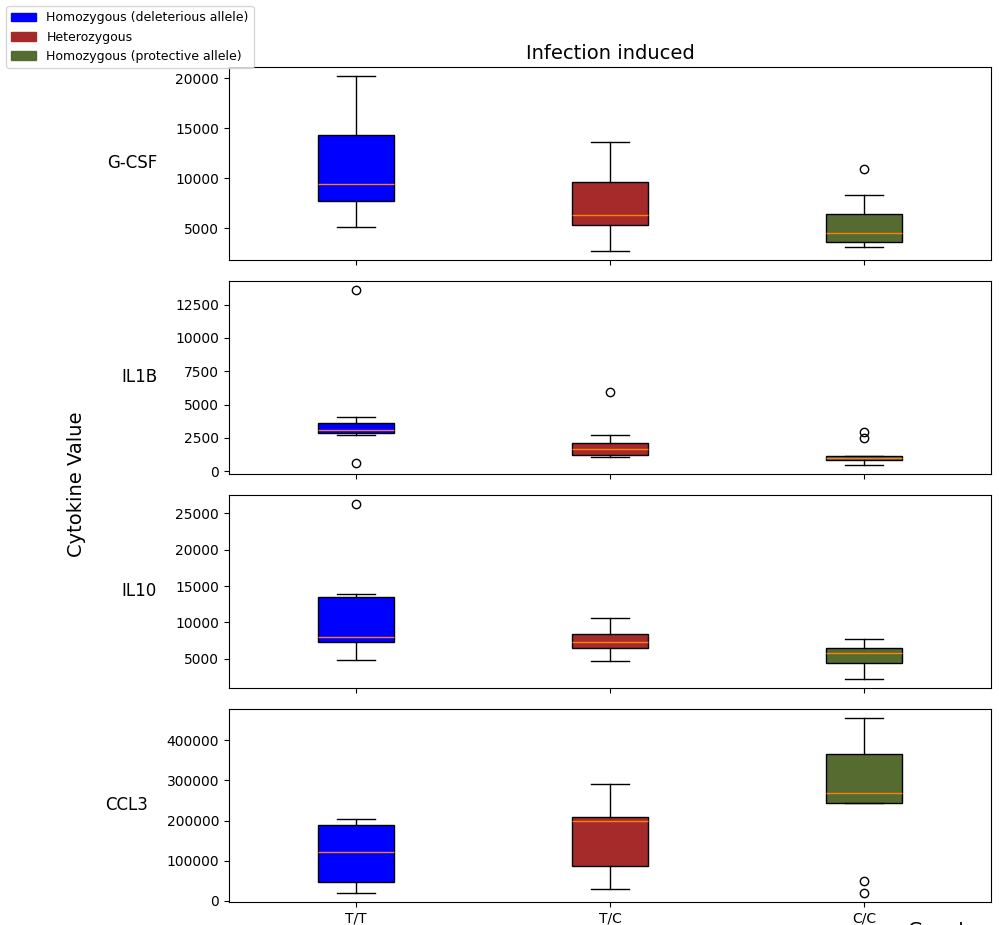
\includegraphics[width=0.5\textwidth]{images/box-plot-detailed.png}
    \caption{ERAP2 vs Cytokine Values (Y.Pestis)}
  \end{figure}
\end{frame}

\begin{frame}
  \frametitle{Predicting effectiveness}
  \begin{itemize}
      \item Use of a linear model to create proportion values
      \item Cytokine Values
  \end{itemize}
\end{frame}

\begin{frame}
  \frametitle{Effectiveness study}
  \centering
  \begin{figure}
    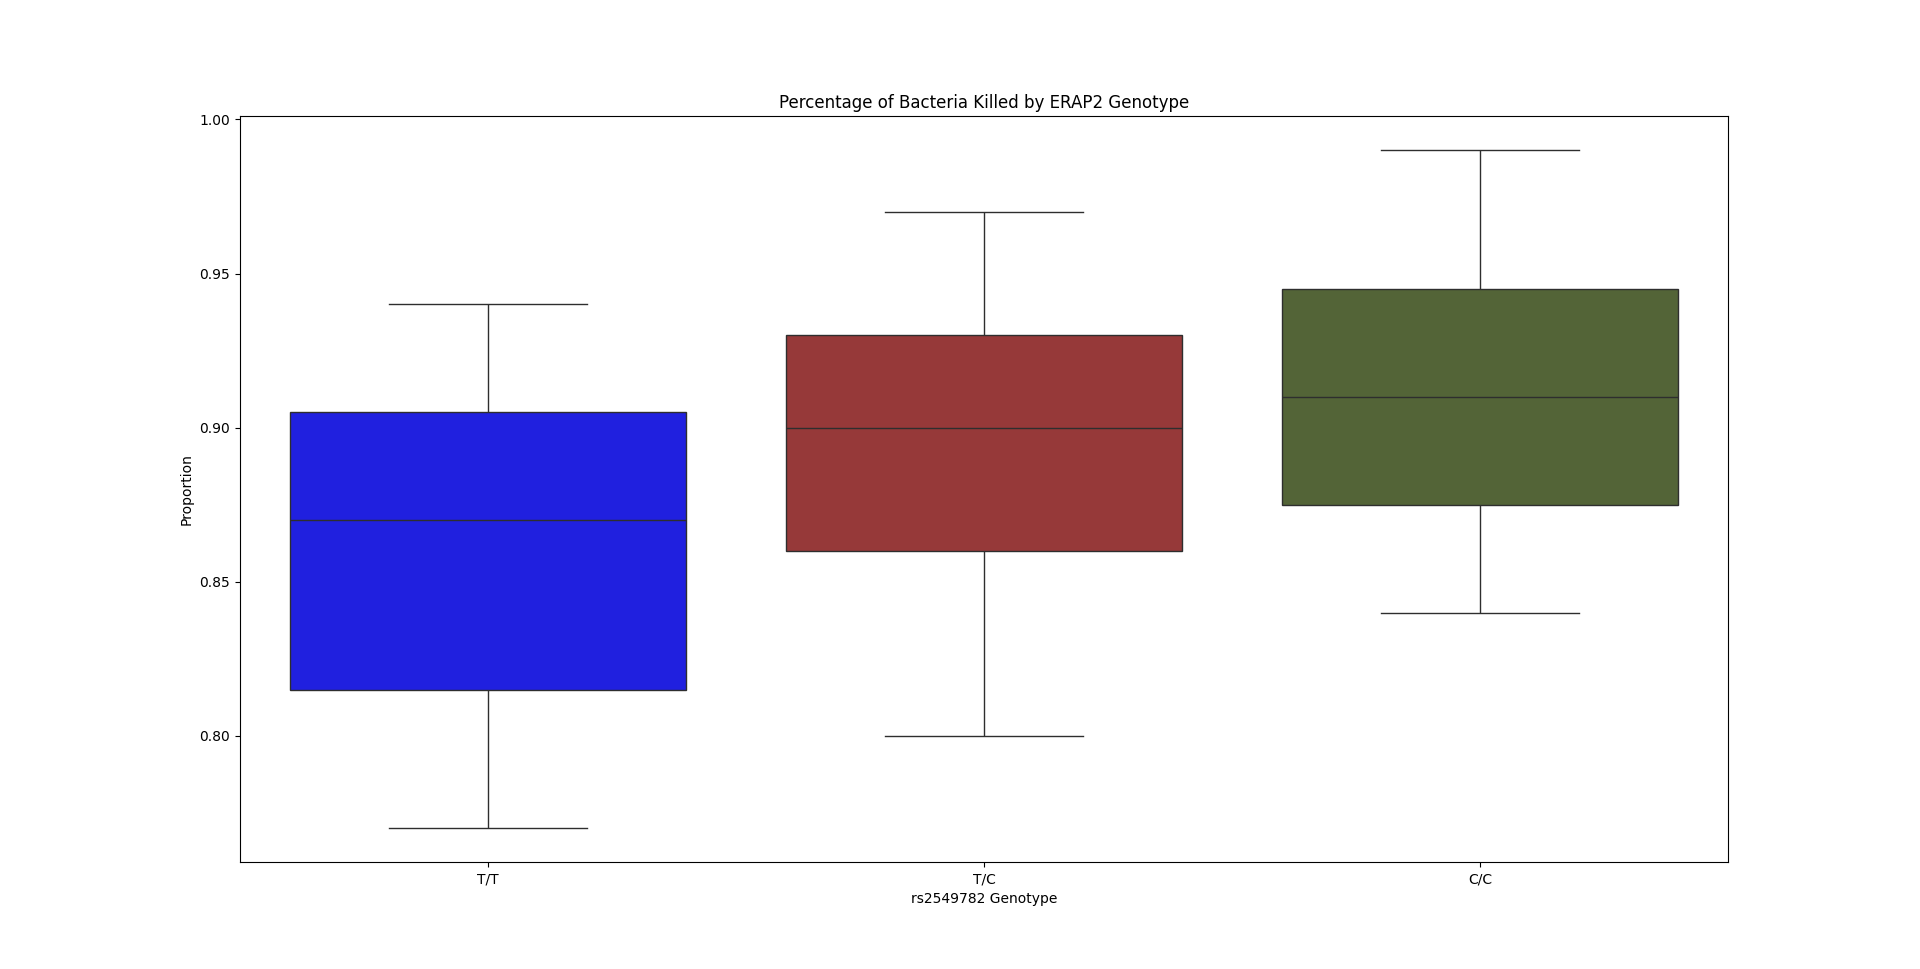
\includegraphics[width=1\textwidth]{images/proportion-genotype.png}
    \caption{proportion bacteria killed vs genotypes}
  \end{figure}
\end{frame}

\begin{frame}
  \frametitle{Further: modern population studies}
  \centering
  \begin{figure}
    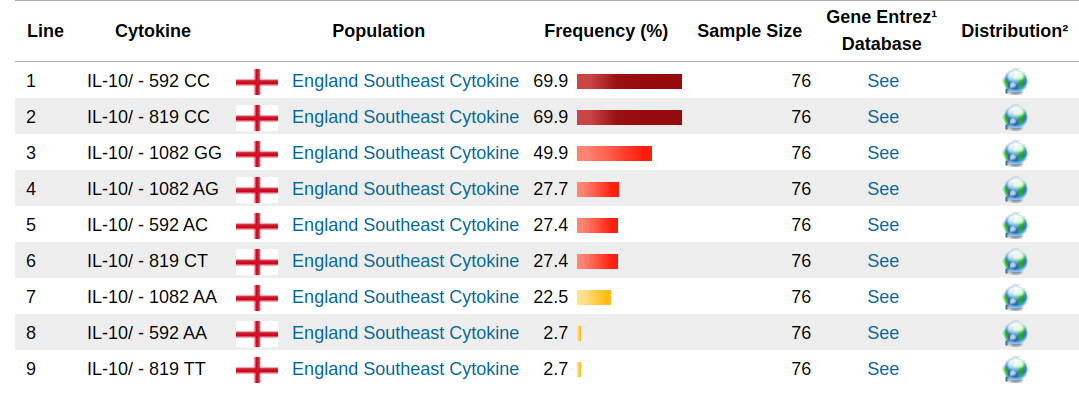
\includegraphics[width=1\textwidth]{images/mod-eng-gen.png}
    \caption{Allele Frequency Net Database}
  \end{figure}
\end{frame}

\begin{frame}
\vspace{6mm}
  \frametitle{How have they changed?}
  \begin{figure}
      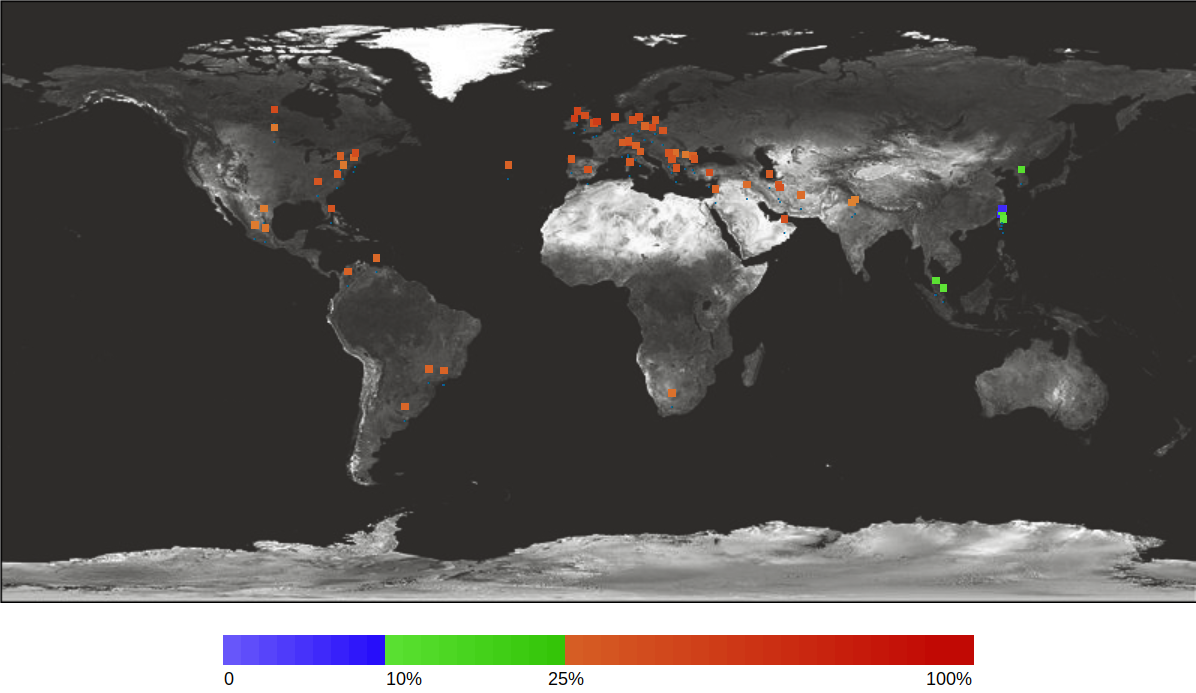
\includegraphics[width=0.31\textwidth]{images/mod-cc.png}
      \caption{Modern Spread - C/C genotypes}
  \end{figure}
  
  \begin{figure}
      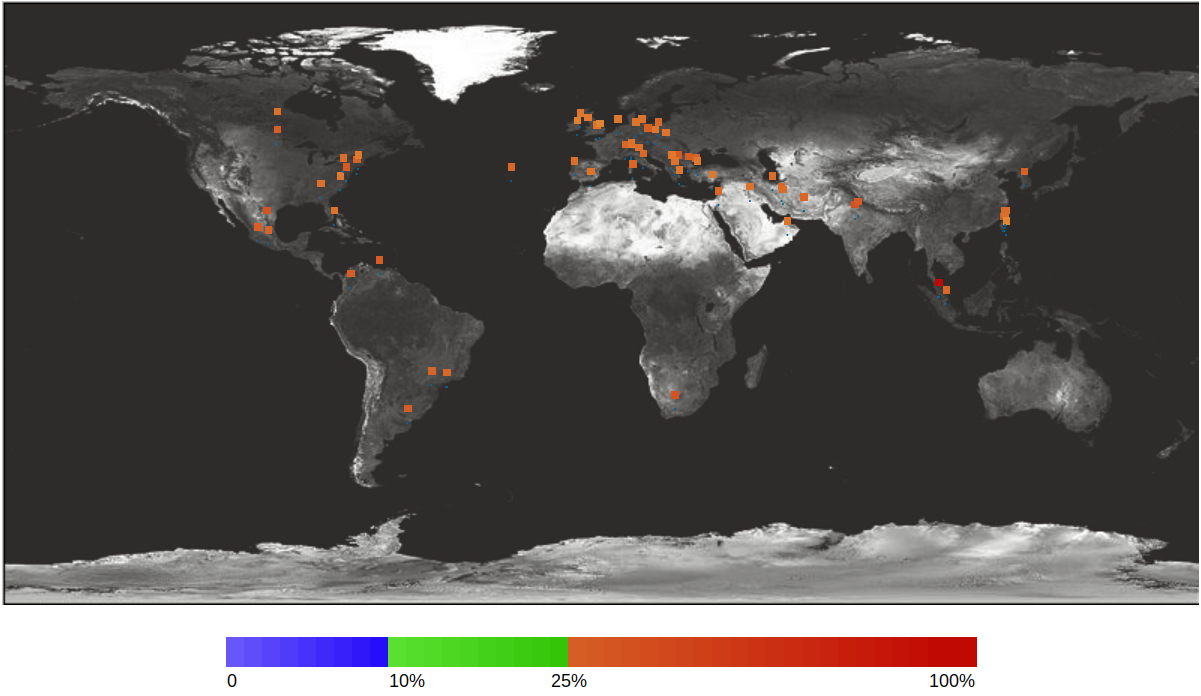
\includegraphics[width=0.31\textwidth]{images/mod-ct.png}
      \caption{Modern Spread - C/T genotypes}
  \end{figure}
\end{frame}

\begin{frame}
  \frametitle{Completely changed...}
  \centering
  \begin{figure}
    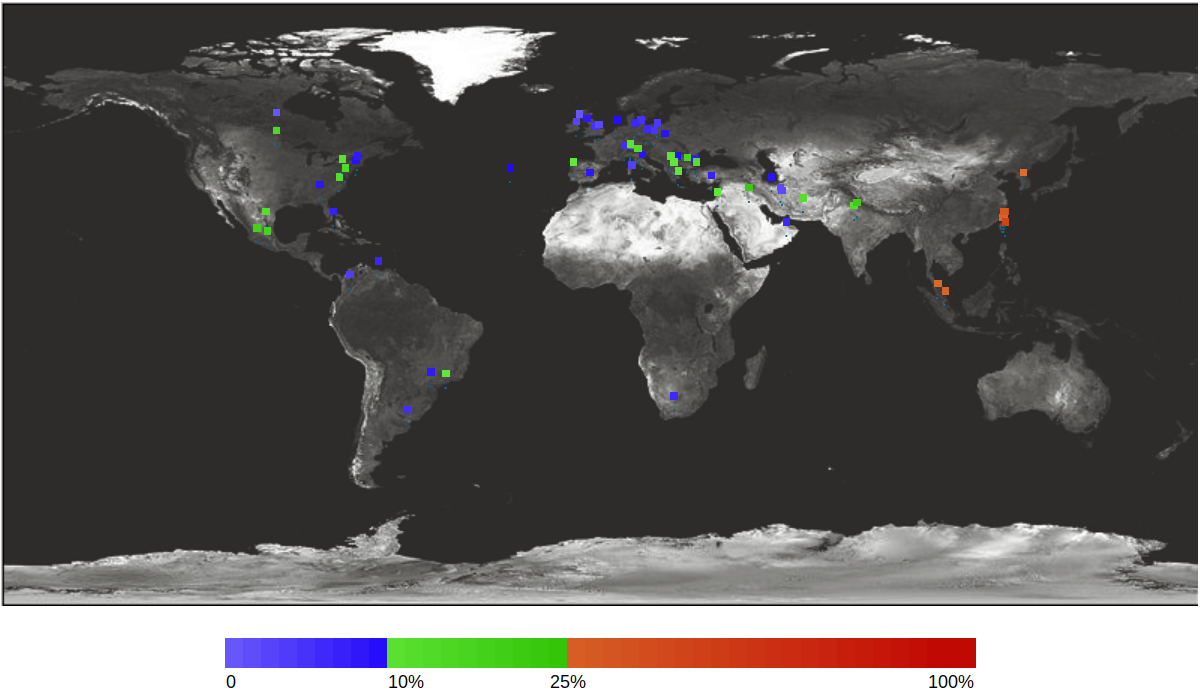
\includegraphics[width=0.8\textwidth]{images/mod-tt.png}
    \caption{Modern Spread - T/T genotypes}
  \end{figure}
\end{frame}

\begin{frame}
  \frametitle{Possible explanations}
  \begin{itemize}
      \item Genetic drift
      \item Population Migration
  \end{itemize}
\end{frame}

\begin{frame}
  \frametitle{Extensions}
  \begin{itemize}
      \item Highlights need for in-depth genomic analysis techniques
      \item Genomic data from other areas in the world
      \item Studies and prevention: medical industry
      \item Disease susceptibility models
  \end{itemize}
\end{frame}

\end{document}
